\documentclass[11pt]{article}
\usepackage{graphicx}
\usepackage{onecolceurws}
\usepackage{hyperref}
\usepackage{float}
\usepackage{caption}
\usepackage{subcaption}
\usepackage{array}

\makeatletter
\def\and{%                  % \begin{tabular}[t]{c}
  \end{tabular}%
  \hskip -0.3em \@plus.17 fil%
  \begin{tabular}[t]{c}}%   % \end{tabular}
\makeatother

\title{Automated similarity detection:\\ identifying duplicated requirements\\\textit{PEC1 - Work plan}}

\author{
%
Quim Motger de la Encarnación
%}
\institution{Universitat Oberta de Catalunya\\Universitat Politecnica de Catalunya}
}

\begin{document}
\maketitle

\section{Introduction}
\label{sec:introduction}

This document is an introductory description of the scope and the work methodology plan for the master thesis titled \textit{``Automated similarity detection: identifying duplicated requirements"}. The following sections aim to present a general depiction of the work plan, starting from the topic proposal and refinement until the elaboration of the final thesis and its defense.

To achieve this purpose, this deliverable is structured in two main sections. The first section contains the development of the thesis topic. It provides a general description of the project proposal, which includes the main topic, the scope of the project, the areas of interest, and the expected results from an academical point of view. Based on this description, it also presents a detailed list of general and specific objectives, which will be used as the general guidelines for the tasks carried out during the thesis development.

The second section addresses the details about the work development methodology and schedule, using the previous details - such as the specific objectives - to extract concrete tasks and evaluate their development from a management perspective. Taking this plan as a reference, it is also necessary to identify possible risks that may affect the success of some of the project goals, as well as to propose mitigation techniques for these risks.

This thesis is being developed as a final master thesis inside the \textit{Computer Engineering Master's degree} program, and therefore it is planned and developed following its quality and evaluation guidelines and deadlines.

\section{Thesis topic}
\label{sec:topic_description}

In this section a general description of the master thesis and the goals of the project are introduced.

\subsection{General description}
\label{sec:general_introduction}

\textbf{Artificial Intelligence} (AI) is a wide-known computer science area which has experienced an exponential growth both in the research field and in real use-case applicability. This computational representation of human cognitive knowledge can be used in many different areas of application, according to the features and the main goals of these fields. Two of the most known areas of AI are \textbf{Machine Learning} (ML) and \textbf{Natural Language Processing} (NLP).

On the one hand ML is a ``general purpose technology"\cite{b8} which uses data and information to learn real-world related knowledge and to improve the reliability of a specific action. Its main application is to use this acquired knowledge to extract autonomous predictions about partial observations of this data. In essence these systems or algorithms differ from traditional programming schemes due to the results accuracy improvement based on its own experience.

On the other hand NLP has a large potential in different applications involving automated, computational processes of all kinds of documents and textual items. This technology applies to the task of developing partial representations of features and rules of natural language based on its textual information, which includes both syntactic and semantic knowledge \cite{b1}.  The main purpose of this technology is to use this representative knowledge in order to apply automated analysis and generation of text units, such as comprehensive sentences or full documents.

One of the areas of application of AI - and more specifically, NLP and ML - is the \textbf{Requirements Engineering} (RE) field. RE is the set of activities and processes of software engineering focused on the development, analysis, communication and management of a set of requirements that describes the features of a system \cite{b2}. Software development experience in recent years proves that managing and maintaining large sets of requirements have become critical issues. This problem is even more challenging due to the large amount of data and the dimensions that these projects are dealing with nowadays \cite{b3}. Whether the analysis and the evaluation of requirements is a tedious, time-consuming task,  it is critical that they are carried out with both accuracy and efficiency in any software development project.

Between the main problems of RE we can highlight the \textbf{detection and management of duplicated requirements} \cite{b4}. If ignored, these duplicated items may lead to redundancy in the textual information of a project and therefore this may lead to the duplicity of tasks, which are critical issues from the project management perspective. Moreover, the automation of this process and the standardized usage of specific, accurate tools are still at a state-of-the-art stage. It is difficult to find open source tools and frameworks providing generic, adaptive solutions for duplicate detection, and most of them are addressed to a very specific casuistic or use case \cite{b5}. In addition to that, similarity detection algorithms are highly tightened to the quality of the data used for the detection process \cite{b6}.

This is the starting point of this master thesis: \textbf{an analysis of the state-of-the-art proposal to apply automated requirements similarity detection}, using artificial intelligence techniques, for the detection of duplicates between project requirements. \textbf{Based on a research of the state-of-the-art, this master thesis must be both a portfolio and a practical evaluation of real duplicate detection algorithms and scenarios in software engineering project requirements. } 

This thesis will be developed within the OpenReq project \cite{b7}, an EU Horizon 2020 project which main goal is \textit{"to build an intelligent recommendation and decision system for community-driven require­ments engineering"}. This collaboration allows the usage of real requirements data to evaluate the similarity detection algorithms developed in this project.

The details about the scope and the goals of the project are depicted in the following sections.

\subsection{General objectives}
\label{sec:main_objectives}

Listed below are the global objectives of the project.

\begin{enumerate}
\item[O1.] \textbf{To research the state-of-the-art of the requirements similarity detection field.} The final thesis document must include a summary of the collected information related to the application of similarity detection in the RE field. The achievement of this goal guarantees the necessary input knowledge to propose and develop the algorithmic tool to evaluate a real duplicated requirements detection scenario.
\item[O2.] \textbf{To develop a requirement similarity-detection multi-algorithm tool.} The main core of the developed software must be the technical implementation of the algorithms selected to be evaluated. This development must satisfy usability and evaluation requirements, so that it is possible to apply an analysis and to extract conclusions from the achieved work.
\item[O3.] \textbf{To define and to evaluate a real application use case for duplicated requirements detection.} As part of the Horizon 2020 OpenReq project, this project will be tested against a real use case dataset from a company - a set of requirements including duplicated and not duplicated items. Therefore, one of the main goals must be setting up the experiment and data preprocess, so the data can be tested with the developed tool. It is important that the experiments execution provide tools and techniques to extract empirical results to evaluate at the end of the project, allowing to conclude the thesis with considerations and validated knowledge on the performance and accuracy of the algorithms.
\end{enumerate}

\subsubsection{Specific objectives}
\label{sec:spec_objectives}

Using the list of global objectives as an input, the specific objectives are listed in the following list.

\begin{enumerate}
\item[O1.1.] To study the current status of similarity detection in the RE field from a general point of view.
\item[O1.2.] To review and to enumerate similarity detection techniques/algorithms, and to be specific the ML and NLP techniques that represent the state-of-the-art of the field.
\item[O1.3.] To identify potential suitable algorithm candidates for the master thesis and the use case to be validated with.
\item[O2.1.] To elaborate a development proposal for the implementation of the selected algorithms.
\item[O2.2.] To integrate the algorithms with a unique tool to use and to test the different similarity detection scenarios.
\item[O3.1] To evaluate the requirements input data of the algorithms, in order to guarantee a comprehensive analysis of the results.
\item[O3.2] To optimize and to adapt the algorithms based on the use case requirements.
\item[O3.3] To analyze and to prepare a use case dataset for all scenarios (i.e. all the different similarity detection algorithms).
\item[O3.4] To carry out the experiments using the developed algorithms.
\item[O3.5] To perform a comparative analysis between algorithms.
\item[O3.6] To extract conclusions in terms of reliability of the results and performance of the algorithms.
\end{enumerate}

\subsection{Master thesis structure}

Based on the specific goals and the scope of the project, below is presented the general structure of the master thesis final document.

\begin{enumerate}
\item Introduction
\begin{enumerate}
\item Project's description and motivation
\item Area of interest and research field introduction
\item Potential stakeholders and applicability
\item General and specific objectives
\item Approach and methodology
\item Work plan
\item Summary of obtained products and results
\item Thesis organization
\end{enumerate}
\item State of the art
\begin{enumerate}
\item Research in similarity detection applied to the RE field
\item Introduction of the OpenReq approach
\item Algorithmic and technical tools for requirements duplicate detection
\item Comparative analysis between algorithms
\end{enumerate}
\item Duplicated requirements detection system
\begin{enumerate}
\item System design and description
\item Development of similarity detection algorithms
\item Integration and software release
\end{enumerate}
\item Experimentation
\begin{enumerate}
\item Use case description: duplicate detection in an issue repository
\item Technical experimentation preparation
\item Results evaluation
\end{enumerate}
\item Conclusions
\begin{enumerate}
\item Objectives achievement
\item General project evaluation
\item Future work
\end{enumerate}
\end{enumerate}

\section{Work plan}

In order to achieve the specific objectives of this thesis, this section introduces the details of the work development methodology. It also includes the list of tasks to carry out and a schedule proposal for its achievement according to the deadlines of the project. For this purpose, a risk identification and a mitigation proposal is also introduced.

\subsection{Development methodology}

This thesis will be developed following a \textbf{Kanban-based methodology} with some general influences from Scrum, which has been proven to be a good approach for projects of this kind of nature (in terms of size and effort) \cite{kanban}. This decision can be justified by three main reasons.

First of all, it seems suitable to propose an agile software development methodology to achieve the goals depicted in this document. Although this project starts from a clear, specific stage, and the objectives are detailed enough, the research of the state-of-the-art phase will deeply condition the specific tasks that will be done during the technical implementation and the evaluation process (i.e. the number and nature of algorithms to be integrated in the tool and evaluated). It is necessary to handle a certain flexibility in terms of requirements and tasks during the project's development. 

Second of all, this methodology aims to provide results in short-term cycles by scheduling fine-grained tasks that guarantee the success of the project's objectives. Following one of the main guidelines of Kanban, which is the visibility and traceability of the tasks, it is intended to provide a dynamic framework that will allow to complete tasks in a short period of time by identifying, detailing and scheduling them according to the general schedule planning of the master thesis (see section \ref{sec:stage}).

Finally, and following with this last criteria of cyclic and iterative results, one of the main goals of this methodology is to hold weekly retrospective and plan meetings, comparable to analog meetings from the Scrum methodology, with the thesis director. These meetings will allow not only a constant review of the work that has been done, but an iterative review of the remaining tasks and the different potential lines of work that might arise during the development of the project. 

\subsubsection{Project management activities}

For achieving and applying the previous methodology plan, it is required to identify and describe the two main artifacts or activities that will guide the project's development.

\begin{itemize}
\item \textbf{Tasks backlog maintenance.} Based on the Scrum task backlog artifact and the task workflow suggestions from Kanban, a project tasks backlog will be used to identify, classify and organize the development of each of the tasks raised during the development of the project. The specific workflow implementation for this project will be as follows:
\begin{center}
\textbf{To Do $\rightarrow$ Analyzing $\rightarrow$ Doing $\rightarrow$ Reviewing $\rightarrow$ Done}
\end{center}
This backlog must be maintained daily according to tasks progress.
\item \textbf{Retrospective and plan meeting.} A regular weekly meeting with the thesis director is proposed to keep track of the general progress of the project. This meeting must include some of the general activities of both the retrospective meeting and the sprint plan meeting from SCRUM \cite{scrum}. Therefore, the length of each sprint is set to 1 week - which is a short period of time, but will be useful to guarantee the achievement of goals and deadlines as scheduled.
\end{itemize}

\subsection{Stage description and tasks}
\label{sec:stage}

A 4-stage project structure plan is proposed with the following structure.

\begin{itemize}
\item \textbf{Plan.} The main goal of these tasks are related to defining a project proposal and to define the main features of its development before starting to develop the core part of the master thesis.

\textit{Tasks}
\begin{enumerate}
\item[P1.] To perform a first, generic research about the area of interest of the master thesis
\item[P2.] To define the topic and scope of the project
\item[P3.] To identify generic and specific goals
\item[P4.] To describe and to justify a work methodology
\item[P5.] To elaborate a schedule planning, according to deadlines and available resources
\item[P6.] To identify risks and to propose mitigation plans
\item[P7.] To structure the master thesis document and periodical deliverables
\end{enumerate}
\item \textbf{Research.} Includes all tasks related to the state-of-the-art review, as well as the study and the analysis of ML/NLP techniques, algorithms and technologies for the similarity detection field.

\textit{Tasks}
\begin{enumerate}
\item[R1.] To research the state-of-the-art of similarity detection in RE field
\item[R2.] To enumerate and to acquire a deep knowledge of the algorithms and techniques of interest for duplicated requirements detection
\item[R3.] To review the state-of-the-art study and developed work from OpenReq project in similarity detection
\item[R4.] To identify a set of potential similarity detection algorithms to be developed 
\item[R5.] To analyze and to compare the set of pre-selected algorithms
\item[R6.] To select those similartiy detection algorithms or techniques for duplicated requirements to be implemented and evaluated
\end{enumerate}
\item \textbf{Development.} Having the knowledge and the information extracted as a result of the \textit{Research} phase, it is possible to start all tasks related to the technical development and implementation of the algorithms and the final software project.

\textit{Tasks}
\begin{enumerate}
\item[D1.] To identify and to study the specific NLP/ML technologies and frameworks used in the different algorithms
\item[D2.] To implement Proof-of-Concept (PoC) software for each algorithm and its techniques
\item[D3.] To validate and to test the scalability of the algorithms for the general UC scenario
\item[D4.] To implement stable, usable versions of the algorithms
\item[D5.] To integrate the implementation of each algorithm within a tool for usage and evaluation purposes
\end{enumerate}
\item \textbf{Experimentation.} Finally, the tool resulted from the \textit{Development} stage must be used to run experiments based on a real use case scenario and to extract useful information about the performance of each algorithm.

\textit{Tasks}
\begin{enumerate}
\item[E1.] To define a set of experiments (i.e., a set of requirements) to test the algorithms
\item[E2.] To describe the measures and stats to use for comparison analysis, which should be useful for both an accuracy and a performance analysis
\item[E3.] To run experiments and to collect results
\item[E4.] To analyze collected data and to extract final conclusions
\end{enumerate}
\end{itemize}

\subsubsection{PEC submissions and content}

In order to supervise and to audit the progress of the project, it is required to submit two follow-up reports prior to the final master thesis submission. These documents will be a guarantee of the achievement of the specific goals and tasks described in this document. The main goals of these reports are:

\begin{enumerate}
\item To detail the development of the project and its current state, identifying and justifying possible changes from the original goals.
\item To review the schedule planning and to justify possible deviation and mitigation activities, if any.
\item To deliver partial results from the developed work.
\end{enumerate}

The structure and the general goals of both reports are quite similar and therefore they do not require significant differentiations. However both reports must be an \textit{As-Is} representation of the project status, and it is necessary to match the master thesis work plan with these deliverables. For this purpose, the content of each report is described below:

\begin{enumerate}
\item \textbf{Report Project development - phase \#1.} \textit{Deadline: November 18th, 2019}

The first report of the project development must include the information related to the following tasks:
\begin{itemize}
\item All tasks of the \textit{Plan} stage finished
\item All tasks of the \textit{Research} stage finished
\item Tasks D1-D2 from the \textit{Development} stage finished or at a final phase
\end{itemize}
\item \textbf{Project development - phase \#2.} \textit{Deadline: December 16th, 2019} 

The second report of the project development must include the information related to the following tasks:\begin{itemize}
\item Tasks D3-D5 from the \textit{Development} stage finished or at a final phase
\item All tasks from the \textit{Experimentation} stage finished
\end{itemize}

\end{enumerate}

If there are any goal changes or schedule deviations during the development of the project related to the tasks reported in each report, these changes will be reflected and properly justified in the documents.

\subsubsection{Gantt chart}

The schedule plan of the stages and tasks detailed in previous sections is presented in figure \ref{fig:gantt}, which is a Gantt diagram representation of the schedule plan per week, from the beginning of the project until the deadline of the second \textit{Project development report} - December 16th. Notice that the submission deadline for the master thesis is on December 31st. However, the original plan is to finish the project two weeks before that deadline for mitigation risk purposes (see section \ref{sec:risk}). In addition, the writing of the master thesis will be done simultaneously and progressively during the development of the project.

\begin{figure}[h]
  \centering
    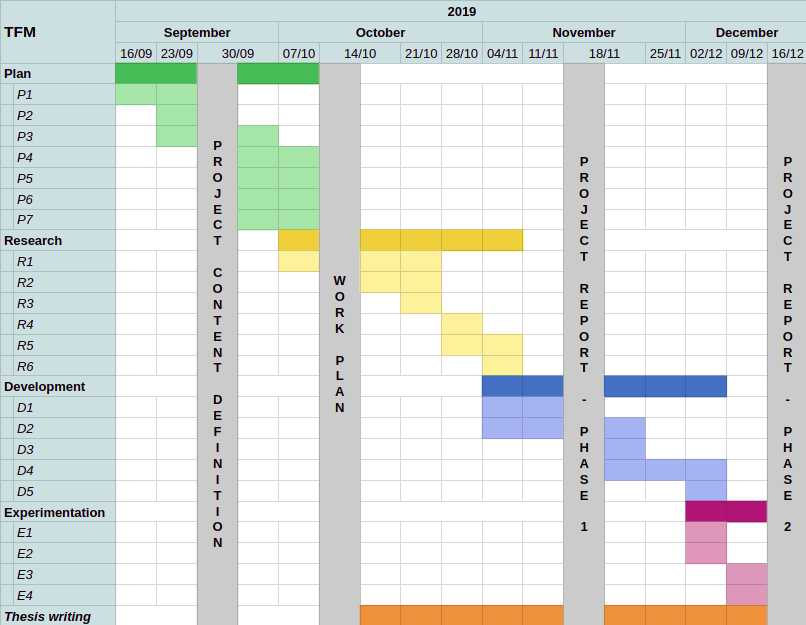
\includegraphics[width=0.8\textwidth]{figures/gantt.png}
      \caption{Gantt diagram of the project's development}
    \label{fig:gantt}
\end{figure}

\subsection{Risk management}
\label{sec:risk}

In this section we identify potential risks that might be raised during the development of the project and a proposal of mitigation activities for reducing the impact of these risks in the achievement of the goals described in sections \ref{sec:main_objectives} and \ref{sec:spec_objectives}.

\begin{itemize}

\item[R1.] \textbf{Deviation of original schedule plan.} It is possible that the estimated time resources for each task may not always be accurate enough, leading to a delay in the completion of tasks and as a consequence a delay on finishing stages on time to keep the project on track.

\textit{Mitigation.} As a preventive measure, to elaborate a stage plan assigning timing resources in a preventive way, dedicating a ratio of extra hours per task and a time period at the end of the project to correct possible delays with respect to the original plan. If this is not enough, to propose a prioritization of specific tasks that will not compromise the achievement of the main goals of the project.

\item[R2.] \textbf{Unexpected obstacles in developing a similarity detection algorithm.} The most critical part of the project is all problems related to the implementation and development of the similarity detection algorithms identified and selected during the \textit{Research} phase. It is possible that some of these algorithms are complex to develop due to different causes, like a lack of knowledge of a specific technology, or the raise of issues or requirements not identified during the state-of-the-art analysis.

\textit{Mitigation.} To analyze in iterative cycles (i.e. during retrospective meetings) the algorithms development viability and evaluate if necessary the possibility to discard or to change the requirements of the project. 

\item[R3.] \textbf{Unexpected results or difficulties in UC evaluation.} It is possible that an algorithm's execution leads to unexpected problems for evaluation purposes, such as a bad estimation of the required resources for its execution. These resources can be conceived as technical resources (i.e., enough RAM) or human/time resources (i.e., its development is more complex than expected, or a single execution requires too much time to be evaluated).

\textit{Mitigation.} As a preventive measure, to dedicate specific effort during the state-of-the-art analysis to understand the nature of the algorithms and to identify the requirements for its execution. If this is not enough and the risk is materialized, an alternate approach would be to reduce the size of experimentation and try to apply a scalar analysis for the real UC application.
\end{itemize}

\begin{thebibliography}{99}

\bibitem{b8} Brynjolfsson, Erik, and Tom Mitchell. “What Can Machine Learning Do? Workforce Implications.” Science. American Association for the Advancement of Science. https://science.sciencemag.org/content/358/6370/1530.
\bibitem{b1} Collobert, Ronan, Jason Weston, León Bottou, Michael Karlen, Koray Kavukcuoglu, and Pavel Kuksa, Natural Language Processing (Almost) from Scratch, Journal of Machine Learning Research, http://www.jmlr.org/papers/volume12/collobert11a/collobert11a.pdf.
\bibitem{b2} Jeremy Dick, Elizabeth Hull, Ken Jackson, Requirements Engineering, Springer, pp. 7–9, ISBN 978-3-319-61073-3
\bibitem{b3} Kasauli, Rashidah, Grischa Liebel, Eric Knauss, Swathi Gopakumar, and Benjamin Kanagwa. Requirements Engineering Challenges in Large-Scale Agile System Development - IEEE Conference Publication. https://ieeexplore.ieee.org/document/8049141.
\bibitem{b4} Natt och Dag, J., Regnell, B., Carlshamre, P. et al, A Feasibility Study of Automated Natural Language Requirements Analysis in Market-Driven Development -  Requirements Eng (2002) 7: 20, https://doi.org/10.1007/s007660200002
\bibitem{b5} Tung Khuat, Nguyen Hung, Le Thi My Hanh, A Comparison of Algorithms used to measure the Similarity between two documents. International Journal of Advanced Research in Computer Engineering \& Technology (IJARCET), https://pdfs.semanticscholar.org/43f8/027780d2694331ca373c57f9a2ace509a7b6.pdf
\bibitem{b6} Yu Huang, Fei Chiang, Refining Duplicate Detection for Improved Data, http://ceur-ws.org/Vol-2038/paper3.pdf
Quality
\bibitem{b7} Requirements Engineering - Tools and Solutions Offered by OpenReq, OpenReq, https://openreq.eu/.
\bibitem{kanban} Kniberg, Henrik, Mattias Skarin, and David Anderson. "Kanban y Scrum–obteniendo lo mejor de ambos." Prólogo de Mary Poppendieck \& David Anderson. ESTADOS UNIDOS DE AMÉRICA: C4Media Inc (2010).
\bibitem{scrum} Schwaber, Ken, and Jeff Sutherland. “The Scrum Guide.” Scrum.org. https://www.scrum.org/resources/scrum-guide.

\end{thebibliography}

\end{document}


